\chapter{Ajuste linear}
\label{chap:minquad}
\section*{Ajuste de uma função linear por Mínimos Quadrados}
\label{sec:minquad}


Se medimos duas variáveis, X e Y, cuja relação sabemos que é linear, podemos encontrar uma relação analítica que melhor ajuste nossos dados. A forma de realizá-la é mediante o procedimento de Mínimos Quadrados, que no caso particular de uma função linear chama-se de regressão ou ajuste linear. Em Física Experimental I, só trabalharemos com este tipo de ajuste, seja porque as relações das grandezas medidas tem uma relação linear ou porque seremos capazes de linearizar relações entre grandezas.

Vamos então nos focalizar só no caso da regressão linear, deixando o caso mais genérico de mínimos quadrados para ser estudado mais para a frente. Na Figura~\ref{fig:ajuste}, mostramos o caso linear. A dispersão dos valores está associada às flutuações dos valores de cada variável. Supomos uma tendência linear entre as variáveis X e Y, e nos perguntamos qual é a melhor reta: 
\begin{equation}
y(x) = a x + b
\end{equation}
\noindent
que ajusta estes dados. A quantidade $y_i - y(x_i)$ representa o desvio de cada medida $y_i$ em relação ao valor previsto pelo modelo $y(x)$.

\begin{figure}[h]
\begin{center}
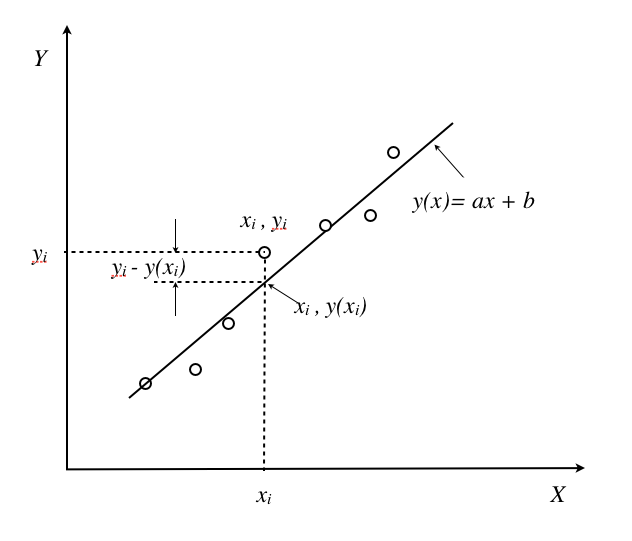
\includegraphics[width=8cm]{fig/GraficoAjusteLin}
\vspace{-0.4cm}
\caption{\label{fig:ajuste} Gráfico de dados associado a um modelo linear.}
\vspace{-1.5cm}
\end{center}
\end{figure}

Vamos definir uma função $\chi^2$ (chi-quadrado), dada por: 
\begin{equation}
\chi^2 = \sum_{i=1}^N (y_i - (ax_i + b))^2
\end{equation}
\noindent
onde $N$ é o número de pontos que serão utilizados para a realização do ajuste linear. Desta forma, a função $\chi^2$ é uma medida do desvio total dos valores medidos $y_i$ em relação aos valores previstos pelo modelo linear $ax + b$. Os melhores valores para o coeficiente angular $a$ e o coeficiente linear $b$ são os que minimizam este desvio total, ou seja o valor de $\chi^2$. Portanto, os melhores valores de $a$ e $b$ serão os que satisfazem:
\begin{equation}
\frac{\partial \chi^2}{\partial a} = 0~~~~~ \text{e}~~~~~ \frac{\partial \chi^2}{\partial b} = 0
\end{equation}

Resolvendo as duas equações obtemos (mostrar):
\begin{equation}
a = \frac{N\sum_i x_i y_i - \sum_i x_i \sum_i y_i}{N \sum_i x_i^2 - (\sum_i x_i)^2}
\end{equation}
\begin{equation}
b = \frac{\sum_i x_i^2 \sum_i y_i - \sum_i x_i \sum_i x_i y_i}{N \sum_i x_i^2 - (\sum_i x_i)^2}
\end{equation}

Estes dois resultados se aplicam ao caso em que todos os dados da variável dependente ($y$) têm a mesma incerteza absoluta e a incerteza da variável independente ($x$) considera-se desprezível. As incertezas dos parâmetros $a$ e $b$ são dadas por:
\begin{equation}
\sigma_a = \sqrt{\frac{\chi_N^2}{N~V[x]}} ~~~~~ \text{e}~~~~~ \sigma_a = \sqrt{\frac{\chi_N^2 \sum_i x_i^2}{N~V[x]}}
\end{equation}
\noindent
onde $V[x]$ é a variância de $x$ e $\chi^2_N$ é conhecido como o chi-quadrado por grau de liberdade (ou chi-quadrado reduzido), que no caso linear está dado por:
\begin{equation}
\chi^2_N = \frac{1}{N-2} \chi^2 = \frac{1}{N-2} \sum_{i=1}^N (y_i - (ax_i + b))^2
\end{equation}

A qualidade do ajuste linear pode ser determinada pelo {\it coeficiente de correlação} dado por:
\begin{equation}
\rho = \frac{\frac{1}{N} \sum_i x_i y_i - \frac{1}{N^2} \sum_i x_i \sum_i y_i}{\sqrt{V[x] V[y]}}
\end{equation}
\noindent
onde:
\begin{equation}
V[x] = \frac{1}{N} \sum_{i=1}^N x_i^2 - \left( \frac{1}{N} \sum_{i=1}^N x_i \right) ^2 ~~~ \text{e}~~~V[y] = \frac{1}{N} \sum_{i=1}^N y_i^2 - \left(  \frac{1}{N} \sum_{i=1}^N y_i \right)^2
\end{equation}



\section*{Método gráfico para ajustar uma reta com incerteza}\label{retagrafico}



Se medimos duas variáveis, X e Y, cuja relação sabemos que é linear, podemos encontrar uma relação analítica que melhor ajuste nossos dados. No Capítulo ~\ref{sec:graf}  da parte Conceitos Básicos na apostila discutimos como isto é feito analiticamente mediante o método de mínimos quadrados, mas aqui estudaremos como faze-lo a partir do gráfico de Y em função de X, o que chamamos de {\bf método gráfico}.

Na Figura~\ref{fig:graflin} podemos observar a distribuição dos dados, círculos abertos, que queremos ajustar. Neste caso, para simplificar, vamos considerar que a incerteza associada a cada medida é do tamanho do ponto.  Para ajustar graficamente os pontos  por uma reta que melhor representa a variação de Y em função de X devemos traçar uma reta de forma tal que os pontos que se situem ``acima" da reta se vejam compensados pelos pontos que se situem ``abaixo'' da mesma, como na linha cheia mostrada na Figura~\ref{fig:graflin}~\footnote{Note que o uso de uma régua transparente é conveniente pois permite ter uma visão global de todos os pontos.}. 
\begin{figure}[!h]
\vspace{-0.4cm}
\begin{center}
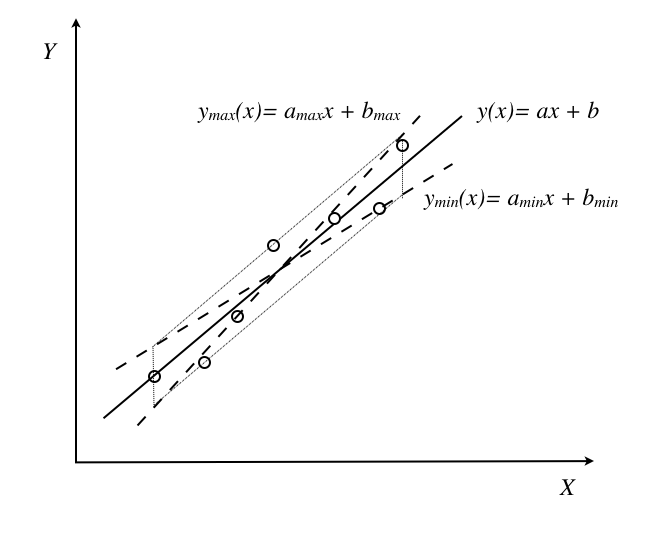
\includegraphics[width=9cm]{fig/GraficoLinGrafico}
\caption{\label{fig:graflin} Método para ajuste linear.}
\vspace{-0.4cm}
\end{center}
\end{figure}


Desta forma podemos determinar o coeficiente angular ($a$) e linear ($b$) para a equação da reta $y = ax + b$.  Mas mesmo no caso gráfico é preciso dar as incertezas associadas à determinação de $a$ e $b$.  Para isto, vamos traçar duas linhas paralelas à melhor reta ($R$) que ajusta os nossos dados encontrados, uma passando pelo ponto mais afastado ``acima'' da reta $R$ e outra pelo ponto mas afastado ``abaixo'' da reta $R$. %, formando o paralelepípedo pontilhado tal como é mostrado na figura. 
Caso exista um ou outro ponto excepcionalmente afastado da reta média poderá não ser considerado pois a probabilidade de corresponder a uma medida incorreta é grande. Obtendo a interseção destas retas por duas retas paralelas ao eixo-y que contêm o primeiro e último ponto experimental representado temos um ``paralelogramo de incerteza" como é mostrado na figura (paralelogramo pontilhado). A partir deste, desenhamos as duas retas diagonais achando o que chamaremos a reta de máxima $y_{max} = a_{max} x + b_{max}$ e a de mínima $y_{min} = a_{min} x + b_{min}$ (ver figura).

A partir destas três retas, podemos então determinar as incertezas associadas para o coeficiente angular $\delta a$ e linear $\delta b$ como:
\[
\delta a = \frac{a_{max} - a_{min}}{2} 
\]
\[
\delta b = \frac{b_{max} - b_{min}}{2}
\]

